\documentclass{article}
\usepackage{fancyhdr}
\usepackage{ctex}
\usepackage{listings}
\usepackage[a4paper, body={18cm,22cm}]{geometry}
\usepackage{amsmath,amssymb,amstext,wasysym,enumerate,graphicx}
\usepackage{float,abstract,booktabs,indentfirst,amsmath}
\usepackage{multirow}
\usepackage{enumitem}
\usepackage{listings}
\usepackage{xcolor}
\usepackage{tabularx}
\usepackage{subfigure}
\usepackage[most]{tcolorbox}
\usepackage{accsupp}
\usepackage[backend=biber,style=numeric]{biblatex}
\usepackage[xetex]{hyperref}
\usetikzlibrary{arrows.meta}
\newcommand\emptyaccsupp[1]{\BeginAccSupp{ActualText={}}#1\EndAccSupp{}}
\setlength{\parindent}{2em}
\renewcommand\arraystretch{1.4}
\setmonofont{FiraCode Nerd Font}
\setCJKmonofont{黑体}
\setmainfont{Times New Roman}
\hypersetup{CJKbookmarks=true,colorlinks=true,citecolor=blue,%
            linkcolor=blue,urlcolor=blue,bookmarksnumbered=true,%
            bookmarksopen=true,breaklinks=true}
\lstset{
    % language = C,
    xleftmargin = 3em,xrightmargin = 3em, aboveskip = 1em,
	backgroundcolor = \color{white}, % 背景色
	basicstyle = \small\ttfamily, % 基本样式 + 小号字体
	rulesepcolor= \color{gray}, % 代码块边框颜色
	breaklines = true, % 代码过长则换行
	numbers = left, % 行号在左侧显示
	numberstyle = \small\emptyaccsupp, % 行号字体
    numbersep = -14pt, 
    keywordstyle=\color{purple}\bfseries, % 关键字颜色
    commentstyle =\color{red!50!green!50!blue!60}, % 注释颜色
    stringstyle = \color{red}, % 字符串颜色
    morekeywords={ASSERT, int64_t, uint32_t},
	frame = shadowbox, % 用(带影子效果)方框框住代码块
	showspaces = false, % 不显示空格
    showstringspaces = false,
	columns = fixed, % 字间距固定
    literate=
        {^+}{{{\color{black}\textbf{+}}\colorbox{green!30}{\phantom{XX}}}}1
        {+\t}{{{\color{black}\textbf{+}}\colorbox{green!30}{\phantom{XX}}}}1,
}

%%%%%%%%%%%%%%%%%%%%%%%%%%%%%%%%%%%%%%%%%%%%%%%%%%%%
\addbibresource{references.bib}
%%%%%%%%%%%%%%%%%%%%%%%%%%%%%%%%%%%%%%%%%%%%%%%%%%%%

%%%%%%%%%%%%%%%%%%%%%%%%%%%%%%%%%%%%%%%%%%%%%%%%%%%%
% contstants
\newcommand{\course}{《数学建模及其MATLAB实现》课程报告}
\newcommand{\titleText}{人工智能与就业率}
\newcommand{\authorName}{李鹏达}
\newcommand{\authorID}{10225101460}
\newcommand{\yearMonth}{2024年12月}
%%%%%%%%%%%%%%%%%%%%%%%%%%%%%%%%%%%%%%%%%%%%%%%%%%%%

\title{\titleText}
\author{\authorName}

% 页眉页脚设置
\pagestyle{fancy}
\fancyhf{}
\fancyhead[L]{\course}
\fancyhead[R]{\titleText}
\fancyfoot[C]{\thepage}

\begin{document}

% title
\begin{titlepage}
    \title{\titleText}
    \author{\authorName}
    \thispagestyle{fancy}
    \fancyfoot{}
    \begin{center}
        \phantom{ }
        \vspace{5cm}
        \\
        
\includegraphics[width=0.9\textwidth]{img/ecnu.png}
        \vspace{1cm}
        \\
        \textbf{\fontsize{22}{36}\selectfont{\heiti \course}} 
        \vspace{2cm}
        \\
        \textbf{\fontsize{20}{26}\selectfont{\heiti \titleText}}  
        \vspace{2cm}
        \\
        \large
        \begin{tabular}{cp{4cm}<{\centering}}
            姓\quad 名:& \authorName \\
            \cline{2-2} \\[-2em]
            学\quad 号:& \authorID \\
            \cline{2-2} \\
        \end{tabular}
        \vspace{2cm}
        \\
        \large \yearMonth
    \end{center}
\end{titlepage}

% abstract
\phantomsection
\centerline{\zihao{-3}\heiti \textbf{摘\quad 要}}
\addcontentsline{toc}{section}{摘要}
\pagenumbering{Roman}

\linespread{1.1}\zihao{-4} 
\bigskip
\kaishu
近年来,人工智能技术的迅速发展和应用对就业率产生了深远影响。本文以经典的Diamond-Mortensen-Pissarides(DMP)失业率模型为基础,结合人工智能技术的影响因素,对劳动力市场的动态平衡进行了建模和分析。研究引入了人工智能职业匹配效率、替代率、新职位创造率等关键参数,构建了包含人工智能因素的失业率模型。通过理论推导和数值模拟,本文探讨了人工智能技术对就业率的正负面影响,以及不同参数组合下劳动力市场的可能演化趋势。研究表明,人工智能技术既可能通过提升职业匹配效率和创造新岗位促进就业,也可能通过岗位替代效应加剧失业。本文为理解人工智能对劳动力市场的长期影响及制定相关政策提供了理论基础和实践参考。
\bigskip

\noindent{\heiti \textbf{关键词:}}
人工智能,就业率,就业市场,DMP模型

\songti
\vspace{2cm}

\noindent{\textit{Abstract---}}%
The rapid development and application of artificial intelligence (AI) have profoundly impacted employment rates. Based on the classical Diamond-Mortensen-Pissarides (DMP) unemployment model, this paper incorporates key AI-related factors to analyze the dynamic equilibrium of the labor market. By introducing parameters such as AI-driven job matching efficiency, substitution rate, and new job creation rate, a modified unemployment model is proposed. Through theoretical derivation and numerical simulation, this study explores the positive and negative effects of AI on employment and examines potential labor market trajectories under different parameter settings. The results indicate that AI can both promote employment by enhancing job matching efficiency and creating new opportunities, while exacerbating unemployment through job displacement. This research provides a theoretical foundation and practical insights for understanding the long-term impact of AI on the labor market and for shaping relevant policy measures.

\bigskip
\noindent{\textit{Keywords---}}%
Artificial intelligence, unemployment model, labor market, DMP model

% 正文
\newpage
\pagenumbering{arabic}
\setcounter{page}{1}

\section{引言}

近年,随着生成式人工智能的飞速发展和以ChatGPT为代表的大语言模型的诞生,人工智能技术已经在各个领域得到了广泛的应用。在此过程中,``人类是否会被人工智能取代?''这个问题也再次成为了人们关注的焦点。

人工智能的对劳动力市场产生的影响已经成为了一个不可回避的话题。国际货币基金组织的一项报告\cite{imf2024ai}指出,人工智能将影响全球近40\%的工作,取代其中一些岗位,而对另一些岗位起到补充作用。在发达经济体中,这一比例甚至高达60\%。

就业率作为衡量劳动力市场健康状况的重要指标,将受到人工智能技术发展的直接影响。因此,我们有必要对人工智能对就业率的影响进行深入研究。

\section{相关工作}

\subsection{失业问题的研究}

经过长期的研究和探索,经济学家对就业问题(或失业问题)形成了很多行之
有效的理论。1958年,A. W. Phillips提出了著名的“菲利普斯曲线”理论\cite{phillips1958relation},指出通货膨胀率与失业率存在交替关系。1963年,Arthur Okun \cite{okun1963potential} 描述了失业率和实际经济增长率之间的关系,表明经济增长不足时失业率会上升。Peter Diamond 等提出了“搜索理论”\cite{diamond1982aggregate} \cite{mortensen1982property},指出劳动市场存在摩擦,招聘和求职的过程需要时间和资源,解释了为什么即使在经济繁荣时期,也会有大量的失业现象。Milton Friedman 等提出了“自然失业率”理论\cite{friedman1995role},认为失业率有一个自然的、不可避免的水平,称为自然失业率。这个失业率是由劳动力市场的结构性和摩擦性因素决定的,并且无法通过短期的政策干预永久性地降低。

这些理论为我们理解失业问题提供了重要的参考,但能否将人工智能技术的发展纳入这些理论框架中,仍然需要进一步的研究。

\subsection{人工智能、自动化与就业}

在此前的一些研究中,学者们已经对人工智能或自动化对就业的影响进行了一些探讨。E. Brynjolfsson 和 A. McAfee 提出了“第二次机器时代”\cite{brynjolfsson2014second}的概念,讨论了技术如何改变生产力、就业和收入分配。C. B. Frey 和 M. A. Osborne\cite{frey2017future} 利用机器学习算法对美国的就业岗位进行了分类,发现47\%的美国就业岗位面临被自动化取代的风险。高技能、创造性岗位的自动化风险相对较低,而低技能的重复性岗位面临较高的威胁。IMF的调查\cite{imf2024ai}指出,在发达经济体、新兴市场和发展中国家,受到人工智能影响的工作岗位预计分别占60\%、40\%和26\%。并且,在大多数情况下,人工智能很可能会加剧总体不平等状况,可能导致劳动者因能否利用人工智能而产生两极分化。2020年,世界经济论坛发布了《未来就业报告》\cite{wef2020futureofjobs},指出到2025年,全球劳动力市场将有8500万个工作岗位被自动化取代,但同时也会创造9700万个新的工作岗位。

这些研究为我们提供了一些关于人工智能对就业的影响的初步认识——人工智能将取代一些重复性、低技能的工作,但也会创造新的工作机会。然而,这些研究大多是基于统计数据和机器学习算法的分析,对于人工智能技术对就业率的影响机制,仍然需要进一步的研究。

\section{问题分析}

为了研究人工智能对就业率的影响,我们需要在现有的就业(失业)率模型的基础上,引入人工智能技术因素,建立新的模型。在此过程中,我们需要考虑以下几个问题:

\begin{enumerate}[label=(\arabic*)]
    \item 人工智能技术的发展对就业率的影响机制是什么?
    \item 人工智能对就业率会产生什么程度的影响?这种影响是正向的还是负向的?
    \item 人工智能对就业率的影响是否具有普遍性?不同国家、不同行业的情况是否有所不同?
\end{enumerate}

\section{建模的假设}

为了简化问题,我们做出以下假设:

\begin{enumerate}[label=(\arabic*)]
    \item 均质性假设:我们假设劳动力市场是均质的,所有劳动者具有相同的技能和素质.
    \item 市场紧张度假设:职位空缺与失业者比率是均一且统一的,即不存在区域性的差异。 
    \item 二元状态假设:劳动者只有两种状态,即就业状态和失业状态。就业率可以简单地用失业率来表示。
\end{enumerate}

\section{符号说明}

\begin{table}[H]
    \centering
    \begin{tabular}{cccc}
        \toprule
        符号 & 说明 & 符号 & 说明 \\
        \midrule
        $u$ & 失业率 & $\mu$ & 职业匹配效率 \\
        $s$ & 离职率 & $\alpha$ & 职业匹配弹性 \\
        $L$ & 劳动力总量 & $v$ & 职位空缺率 \\
        $U$ & 失业者数量 & $\theta$ & 劳动力市场的紧张度 \\
        $M$ & 成功匹配数 & $f$ & 匹配率\\
        $V$ & 职位空缺数量 & $g$ & 职位填补率 \\
        $\epsilon$ & 人工智能离职参数 & $\rho$ & 人工智能替代率 \\
        $k$ & 人工智能职业匹配效率参数 & $\gamma$ & 人工智能新职位创造参数 \\
        \bottomrule
    \end{tabular}
    \caption{符号说明}
\end{table}

\section{数学模型建立}

\subsection{简化的Diamond-Mortensen-Pissarides失业率模型}

Diamond-Mortensen-Pissarides(DMP)模型\cite{diamond1982aggregate}\cite{mortensen1982property}是一种经典的劳动力市场模型,用于解释失业率的形成机制。首先,我们建立一个简化的DMP模型,用于描述在未引入人工智能技术的情况下,劳动力市场的运行机制。

在 DMP 模型中,劳动力市场由两类经济主体组成:劳动者和雇主。劳动者在劳动力市场中寻找工作,而雇主则提供工作岗位。
失业者$U$与职位空缺$V$之间的匹配可以通过以下方程描述:
\begin{equation}
    M(U, V) = \mu U^\alpha V^{1-\alpha}
\end{equation}
其中,$M(U, V)$ 表示成功匹配的数量,$\mu$ 是职业匹配效率,$\alpha$ 是职业匹配弹性。
\begin{figure}[htbp]
    \centering
    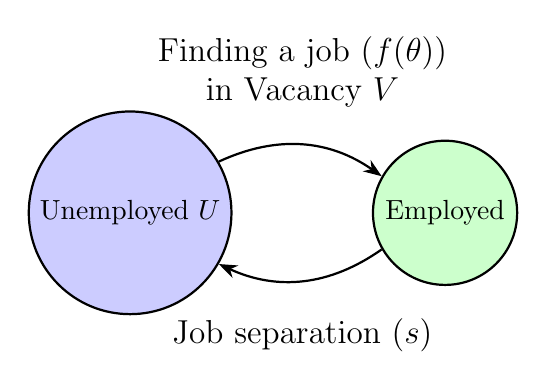
\begin{tikzpicture}[
        node distance=4cm,
        every path/.style={thick, ->, >=Stealth}
    ]
    \node[fill=blue!20, circle, draw] (unemployed) {Unemployed $U$};
    \node[fill=green!20, right of=unemployed, circle, draw] (employed) {Employed};
    \draw[->, bend left=30, text width=3.7cm, align=center] (unemployed) to node[midway, above=1em, font=\large] {Finding a job ($f(\theta)$) in Vacancy $V$} (employed);
    \draw[->, bend left=30] (employed) to node[midway, below=1em, font=\large] {Job separation ($s$)} (unemployed);
    \end{tikzpicture}
    \caption{简化的Diamond-Mortensen-Pissarides模型}
    \label{fig:dmp}
\end{figure}
如图 \ref{fig:dmp} 所示,劳动者在失业状态和就业状态之间转换,失业者在职位空缺中找到工作的概率由 $f(\theta)$ 表示,职位得到填补的概率由 $g(\theta)$ 表示。定义市场的紧张度 $\theta = U / V$,则有:
\begin{equation}
    f(\theta) = \frac{M(U, V)}{U} = \mu U^{\alpha-1} V^{1-\alpha} = \mu \theta^{\alpha-1}
\end{equation}
\begin{equation}
    g(\theta) = \frac{M(U, V)}{V} = \mu U^\alpha V^{-\alpha} = \mu \theta^{\alpha}
\end{equation}
失业率 $u$ 的变化由离职率 $s$ 和失业者找到工作的概率 $f$ 两部分决定,可以由以下微分方程描述:
\begin{equation}
    \dot{u} = s(1 - u) - f(\theta) u = s(1 - u) - \mu \theta^{\alpha-1} u
    \label{eq:dmp}
\end{equation}

考察微分方程 \eqref{eq:dmp} 的平衡点,即 $\dot{u} = 0$,可得:
\begin{equation}
    u^* = \frac{s}{s + \mu \theta^{\alpha-1}}
\end{equation}
令 $F(u) = s(1 - u) - f(\theta) u$,则有 $F'(u^*) = -s - f(\theta) < 0$,即 $u^*$ 是一个稳定的平衡点。这说明,在此模型中,失业率 $u$ 最终会在一个稳定的水平上波动,受到离职率 $s$ 和市场紧张度 $\theta$ 的影响。

\subsection{引入人工智能参数的简化DMP模型}

在上述简化的DMP模型的基础上,我们引入人工智能技术参数,建立新的模型。

随着人工智能应用程度的增加,人工智能辅助的职业匹配将使劳动力市场的职业匹配效率 $\mu$ 会发生变化。我们假设 $\mu'$ 为:
\begin{equation}
    \mu' = (1 + k)\mu
\end{equation}
其中,$k$ 是人工智能职业匹配效率参数,$k > 0$ 表示人工智能技术的应用会提高劳动力市场的职业匹配效率。

在人工智能引入后,空余岗位数量 $V$ 会发生变化,一方面,人工智能技术会取代一部分工作,导致空余岗位数量减少;另一方面,人工智能技术也会创造新的工作机会,增加空余岗位数量。
我们假设人工智能替代率为 $\rho$,则有:
\begin{equation}
    V' = (1 - \rho)(1 + \gamma) V
\end{equation}
其中,$\gamma$ 是人工智能新职位创造参数,$\gamma > 0$ 表示人工智能技术的应用会增加劳动力市场的空余岗位数量。此外,市场的紧张度 $\theta$ 也会发生变化:
\begin{equation}
    \theta' = \frac{U}{V'} = \frac{U}{(1 - \rho)(1 + \gamma) V} = \frac{\theta}{(1 - \rho)(1 + \gamma)}
\end{equation}

人工智能技术的应用也会影响劳动力市场的离职率 $s$,人工智能对工作的替代会导致一部分劳动者失去工作,从而增加离职率。我们假设离职率 $s'$ 为:
\begin{equation}
    s' = (1 + \epsilon)s
\end{equation}

在引入人工智能参数后,失业率 $u$ 的变化由以下微分方程描述:
\begin{equation}
    \dot{u} = s'(1 - u) - f(\theta') u = (1 + \epsilon)s(1 - u) - (1 + k)\mu \left(\frac{\theta}{(1 - \rho)(1 + \gamma)}\right)^{\alpha-1} u 
\end{equation}
其稳定平衡点为:
\begin{equation}
    u^* = \frac{(1 + \epsilon)s}{(1 + \epsilon)s + (1 + k)\mu \left(\frac{\theta}{(1 - \rho)(1 + \gamma)}\right)^{\alpha-1}}
\end{equation}

\subsection{人工智能对单一国家就业率的影响}

在上述模型的基础上,我们可以进一步考虑人工智能对国家就业率的影响。我们假设国家不同行业的劳动力市场的参数不同,即 $\mu$、$s$、$\rho$、$\gamma$、$k$、$\epsilon$ 等参数在不同行业之间存在差异。

设 $u_i$ 为第 $i$ 个行业的失业率,$L_i$ 为第 $i$ 个行业的劳动力总量,$U_i$ 为第 $i$ 个行业的失业者数量,$V_i$ 为第 $i$ 个行业的职位空缺数量,$\theta_i$ 为第 $i$ 个行业的市场紧张度。则有:
\begin{equation}
    \dot{u_i} = (1 + \epsilon_i)s_i(1 - u_i) - (1 + k_i)\mu_i \left(\frac{\theta_i}{(1 - \rho_i)(1 + \gamma_i)}\right)^{\alpha-1} u_i
\end{equation}
国家平均失业率 $\bar{u}$ 可以由各行业失业率的加权平均得到:
\begin{equation}
    \bar{u} = \frac{\sum_{i=1}^n L_i u_i}{\sum_{i=1}^n L_i}
\end{equation}

\section{结果与比较}

在建立的模型中,我们可以通过数值模拟的方法,研究人工智能对就业率的影响。

\subsection{简化的DMP模型}

在简化的DMP模型中,考虑不同的市场紧张度 $\theta$和离职率 $s$ 对失业率的影响。如图 \ref{fig:simple_dmp} 所示,可以看到,市场紧张度 $\theta$ 或离职率 $s$ 越大,失业率 $u$ 越高。

\begin{figure}[H]
\centering
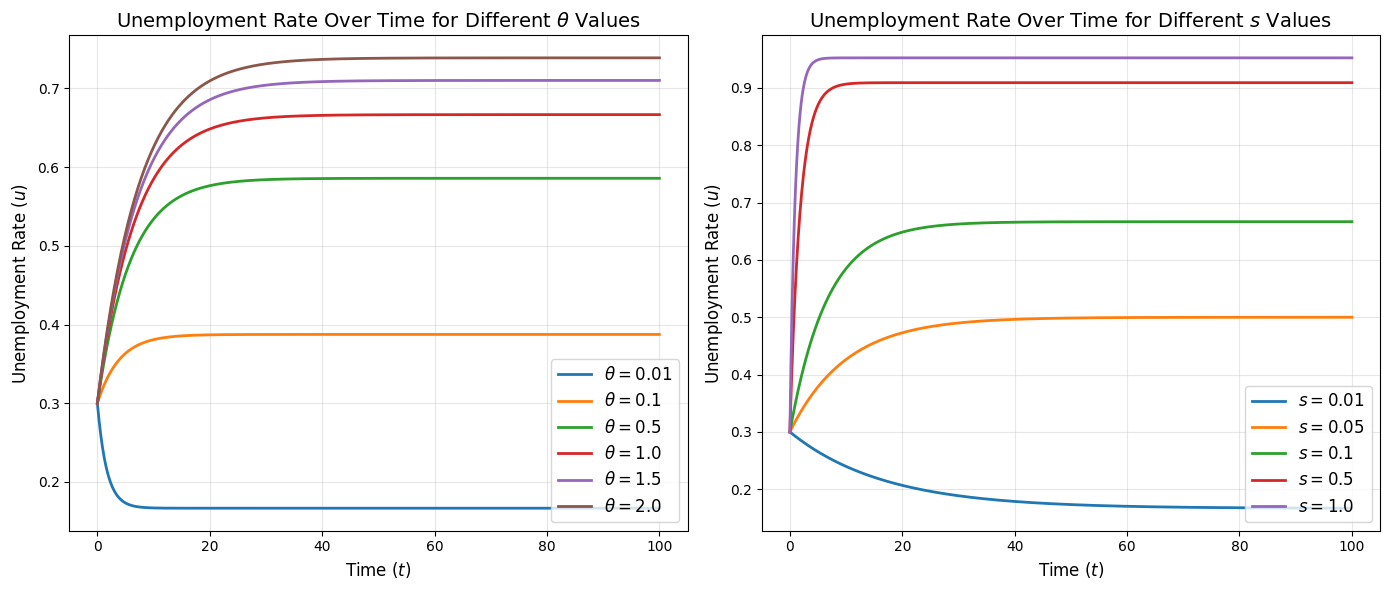
\includegraphics[width=0.9\textwidth]{img/simple_dmp.png}
\caption{简化的DMP模型中失业率随市场紧张度和离职率的变化}
\label{fig:simple_dmp}
\end{figure}

\subsection{引入人工智能参数的简化DMP模型}

在引入人工智能参数的简化DMP模型中,我们可以考虑不同的人工智能参数对失业率的影响。根据不同参数的影响,我们可以将职业按照特点分成以下几类:

\begin{enumerate}[label=(\arabic*)]
    \item AI替代型职业
    
    \begin{itemize}
        \item 特点:人工智能技术的应用会大量取代工作,同时并不能提供新就业岗位,$\rho$ 较大, $\gamma$ 较小;因逐渐被人工智能取代,离职率增加,$\epsilon$ 较大;行业收缩, 职业匹配效率下降,$k$ 为负数。
        \item 示例:数据录入员,快递分拣员
    \end{itemize}

    \item AI驱动型新兴职业
    
    \begin{itemize}
        \item 特点:人工智能技术的应用创造大量工作机会,AI驱动型产业,替代率极低,$\rho$ 极小, $\gamma$ 较大;离职率降低,$\epsilon$ 为负数;职业匹配效率提升,$k$ 较大。
        \item 示例:AI工程师,数据科学家
    \end{itemize}
    
    \item 适应性变革型职业
    
    \begin{itemize}
        \item 特点:人工智能技术的应用会取代部分工作,但也会创造新的工作机会,$\rho$ 和 $\gamma$ 均为中等水平;离职率增加,$\epsilon$ 较大;职业匹配效率提升,$k$ 较大。
        \item 示例:销售员,客服人员
    \end{itemize}

    \item 低AI影响职业
    
    \begin{itemize}
        \item 特点:人工智能技术的应用对工作影响较小,$\rho$ 和 $\gamma$ 均为极小;离职率无显著变化,$\epsilon$ 接近0;劳动市场稳定,职业匹配效率提升,$k$ 较大。
        \item 示例:厨师,保洁员
    \end{itemize}

    \item AI辅助型职业
    
    \begin{itemize}
        \item 特点:人工智能技术的应用会提高工作效率,但难以取代工作,$\rho$ 较小, $\gamma$ 中等;离职率较低,$\epsilon$ 较小;职业匹配效率提升,$k$ 较大。
        \item 示例:医生,律师
    \end{itemize}
\end{enumerate}

\begin{figure}[H]
    \centering
    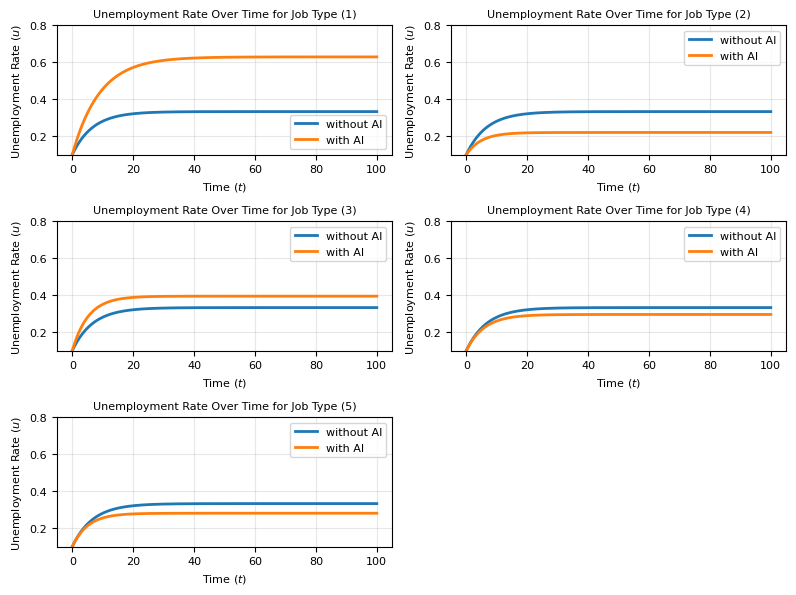
\includegraphics[width=0.9\textwidth]{img/dmp_ai.png}
    \caption{引入人工智能参数的简化DMP模型中不同类型职业的失业率及比较}
    \label{fig:dmp_ai}
\end{figure}

如图 \ref{fig:dmp_ai} 所示,不同类型的职业在引入人工智能参数后,失业率的变化情况。可以看到,AI替代型职业由于人工智能技术的应用,失业率显著增加;AI驱动型新兴职业由于人工智能技术的创新,失业率显著降低;适应性变革型职业和AI辅助型职业的失业率变化较小;低AI影响职业的失业率保持稳定。

\subsection{人工智能对单一国家就业率的影响}

在考虑不同行业的劳动力市场参数后,我们可以进一步研究人工智能对单一国家就业率的影响。

以美国为例,根据美国经济分析局2023年GDP数据\cite{bea2023gdp},我们可以将美国劳动力市场的各行业按照其对人工智能的依赖程度分为不同类型,如表 \ref{tab:gdp_classification} 所示。

\begin{table}[h!]
    \centering
    \begin{tabular}{p{5cm}p{6cm}p{2cm}}
    \toprule
    \textbf{职业分类} & \textbf{对应行业} & \textbf{GDP占比} \\
    \midrule
    AI替代型职业 & 零售贸易、运输和仓储 & 9.9\% \\
    AI驱动型新兴职业 & 信息、专业和商业服务 & 18.4\% \\
    适应性变革型职业 & 制造业、艺术、娱乐、住宿和食品服务 & 14.8\% \\
    低AI影响职业 & 农业、林业、渔业和狩猎、教育服务、医疗保健和社会援助 & 9.5\% \\
    AI辅助型职业 & 金融、保险、不动产、租赁和租赁,政府,建筑 & 36.5\% \\
    \bottomrule
    \end{tabular}
    \caption{美国各职业分类对应行业及其GDP占比}
    \label{tab:gdp_classification}
\end{table}

根据我们先前建立的模型和对各行业的分类,在没有足量数据拟合的情况下,我们可以简单地进行定性分析——人工智能带来的技术变革将在最终稳定后对美国整体就业率产生一定的积极影响,但在此之前,由于技术的不断变革和恐慌情绪的蔓延,失业率将会有所波动。

\section{结论}
本文通过扩展经典的Diamond-Mortensen-Pissarides(DMP)失业率模型,尝试研究人工智能技术对就业率的影响机制。基于简化的模型,我们引入了人工智能相关的参数,包括职业匹配效率参数、替代率和新职位创造参数,并分析了这些参数对劳动力市场动态的影响。

研究表明,人工智能技术的发展对就业率的影响具有双重性。一方面,人工智能通过提高职业匹配效率和创造新职位,能够促进劳动力市场的流动性,从而降低失业率;另一方面,人工智能的替代效应可能导致部分劳动者失业,进而增加整体失业率的风险。这种影响的具体程度取决于人工智能技术的应用深度、行业分布以及劳动力市场的适应能力。

未来的研究可以进一步结合具体行业或地区的数据,通过深度学习等方法拟合本文模型,并探索更多影响人工智能与就业关系的潜在因素,为制定相关政策提供科学依据。

\section{问题}

在研究过程中,我们发现以下新的问题和模型的改进空间:

\begin{enumerate}[label=(\arabic*)]
    \item 政策与市场调节的作用未纳入
    
    政府政策、社会保障体系和劳动者再培训机制等对人工智能技术冲击的缓解作用在本研究中未被充分考虑。这些政策变量在现实中可能显著影响失业率的变化趋势,未来研究可以进一步将政策干预的动态效应纳入模型分析。

    \item 数据驱动模型的引入
    
    人工智能的大范围应用距今时间较短,相关数据的收集和整理工作尚未完全完成。本研究主要基于理论模型推导,缺乏真实数据的支撑。未来研究可以结合实际经济数据,利用机器学习技术构建数据驱动的混合模型,验证理论模型的有效性并优化参数设定。

    \item 二元状态假设的拓展
    
    本研究中,我们假设劳动者只有就业和失业两种状态,未考虑劳动力市场中其他可能存在的状态。未来研究可以进一步拓展模型,引入更多状态变量,如劳动力市场的灵活就业、自由职业等状态,以更全面地分析人工智能对就业率的影响。
\end{enumerate}

\newpage
\phantomsection
\addcontentsline{toc}{section}{参考文献}
\printbibliography[title={\zihao{-3} \heiti \centering 参\ 考\ 文\ 献}]


\end{document}

